\chapter{Performance Evaluation}
\section{Maximum System Efficiency and Minimum Access Delay} 	\label{sec_max_min}
With the system efficiency given in equation \ref{eff_def}, we take the derivative with respect to $\tau$, and find the extreme point, $\tau^\star = M/n$. Since $\tau\in [0,1]$, $\tau^\star = min\lbrace 1,M/n\rbrace$. 
What we care is when $n$, the number of contending stations, is large, i.e., $\tau^\star = M/n$. 
Then the system efficiency is
\begin{align}
\textit{eff}\ (\tau^\star) = (1-\frac{1}{n})^{n-1} 
\end{align}
Then the maximum $n_s$ is easy to generate.
\begin{align}
\label{equ_max_ns}
E[n_s]^\star = M \cdot \textit{eff}\ (\tau^\star) = M(1-\frac{1}{n})^{n-1} 
\end{align}

And the limit on $n$ is
\begin{align}
\label{eff_limit}
\lim_{n\rightarrow \infty}\textit{eff}\ (\tau^\star) = \lim_{n\rightarrow \infty}(1-\frac{1}{n})^{n-1} =\frac{1}{e} 
\end{align}

\begin{figure}[!ht]
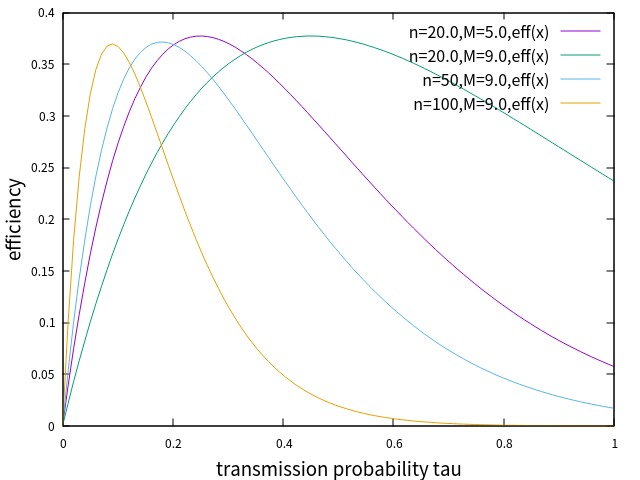
\includegraphics[scale=0.54]{./figure/eff_tau.png}
\caption{Efficiency versus transmission probability $\tau$}
\label{fig_eff_def}
\end{figure}

\begin{figure}[!ht]
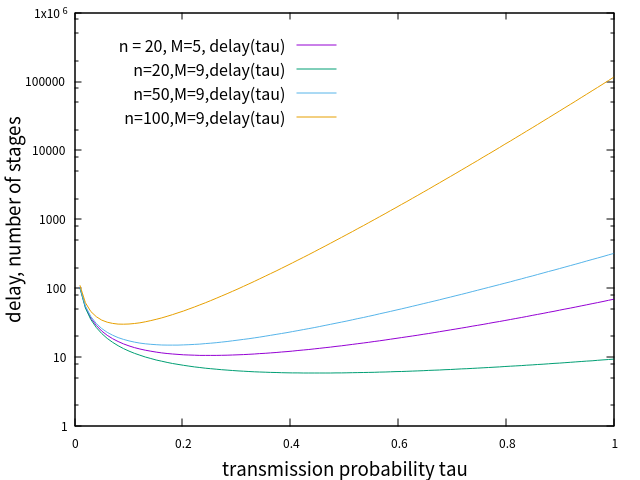
\includegraphics[scale=.54]{./figure/delay_tau.png}
\caption{Access delay versus transmission probability $\tau$}
\label{fig_delay_def}
\end{figure}

With the delay analysis given in \ref{equ_delay}, we also take the derivative with respect to $\tau$, and find the extreme point, $\tau^\star = M/n$. Again, $\tau^\star = min\lbrace 1, M/n\rbrace$. 
When $n\geq M$, the minimum access delay is 
\begin{align}
\label{equ_min_delay}
D(\tau^\star) = \frac{n}{M(1-\frac{1}{n})^{n-1}}.
\end{align}

From above analysis, we find that the maximum system efficiency and minimum access delay are both obtained by the same transmission probability $\tau = min\lbrace 1, M/n\rbrace$.
What's more, system efficiency is independent with $M$, number of RUs for random access in a stage, while $M$ affects access delay. 
The larger $M$ is, the shorter the access delay will be. 
It indicates that when AP allocates RUs for random access, the AP could allocates as many as possible, only if the channel of the RU is sensed idle. 
This rule will be more explained in next section.

Figure \ref{fig_eff_def} and figure \ref{fig_delay_def} are plotted corresponding to equation \ref{eff_def} and \ref{equ_delay} respectively.
Consistent to the analysis above, the figure shows that the maximum system efficiency is independent of number of RUs for random access when $n\geq M$, and approaching to $1/e$ with $n$ increasing. 
What's more, the optimal transmission probability $\tau$ of system efficiency and access delay is consistent with each other, which also validates the analysis. 

According to equation \ref{tau_general} and \ref{p_ax}, transmission probability $\tau$ is dependent on system parameters, $m$, backoff levels, $M$, RUs for random access in a stage, $W_0$, the initial contention window and $n$, number of stations in the network.
The only way to approach optimal performance is to employ adaptive techniques to tune the values $m$, $M$ and $W$ on the basis of the estimated value of $n$.
In the following section, we will evaluate the performance corresponding to different system parameters sets and propose the rules to tune the system parameter sets so that the transmission probability $\tau$ approach the optimal transmission probability, $\tau^\star$, which means both system efficiency and delay approach the optimal. 

\section{Rules of Parameter Configuration} 	\label{sec_perf_eval}
We have estimated the maximum system efficiency and minimum access delay in the previous section. Then we evaluate the metrics, number of stations who succeed in contending in a stage, system efficiency and access delay, under various parameter sets. 
Equally, we could evaluates transmission probability under various parameter sets, since the optimal transmission probability $\tau^\star$ means both maximum system efficiency and minimal access delay.

At last, we propose rules for configuring the parameter set $\lbrace M,m, OCW_{min}\rbrace$.

\subsection{RUs for Random Access $M$}
The analysis above has indicated that $M$, the number of RUs for random access, only affects the minimum access delay, having nothing to do with maximum system efficiency. 
And the bigger $M$ is, the better the performance will be. We will give more explanations here. 

In figure \ref{fig_n_M_eff}, the maximum system efficiency is almost the same. 
The difference is "when" the optimal point will be. 
For larger $M$, the optimal number of stations is larger. It is intuitive.

\begin{figure}[!ht]
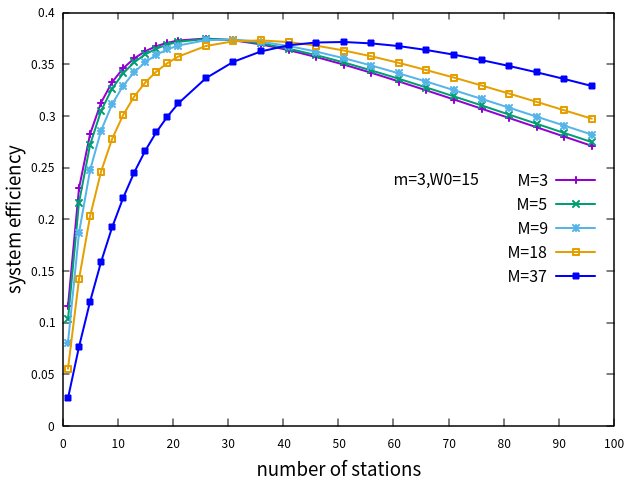
\includegraphics[scale=.54]{./figure/n_M_eff_perf.png}
\caption{System efficiency versus number of stations}
\label{fig_n_M_eff}
\end{figure}

In figure \ref{fig_n_M_delay}, the larger $M$ will linearly decrease the access delay of station. The figure is consistent with the equation \ref{equ_min_delay}. 

\begin{figure}[!ht]
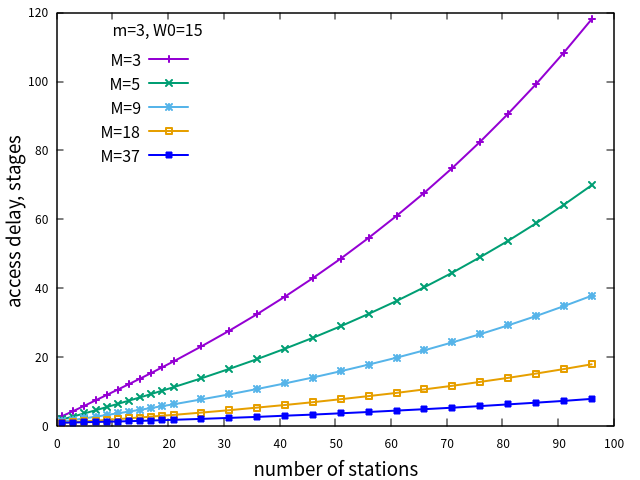
\includegraphics[scale=.54]{./figure/n_M_delay_perf.png}
\caption{Access delay versus number of stations}
\label{fig_n_M_delay}
\end{figure}

More practically, we present the number of successful stations in a single stage versus number of stations in figure \ref{fig_n_M_ns}.
While the maximum system efficiency is the same with different $M$, the actually number of stations who succeed contending in a single stage is much different, which corresponds to equation \ref{equ_max_ns}. 
The optimal value of number of successful stations in a single stage is propotional to $M$. 
Above all, when AP allocates RUs for random access, the AP will sense channels first then allocates as many RUs, which are sensed idle, for random access as possible.

\begin{figure}[!ht]
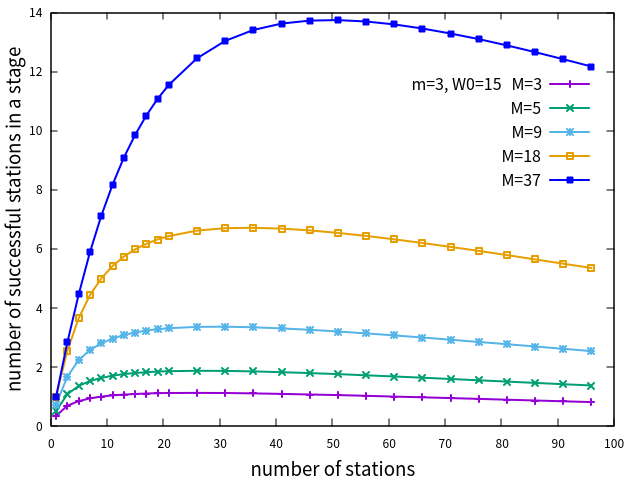
\includegraphics[scale=.54]{./figure/n_M_ns_perf.png}
\caption{Number of successful stations in a single stage versus number of stations}
\label{fig_n_M_ns}
\end{figure}

\subsection{Initial Contention Window $OCW_{min}$, backoff level $m$}
Different from legacy 802.11, the backoff level and initial contention window are allocated as a RAPS element in beacon frame by AP in real time according to the system state, especially number of stations in a BSS.
With the $M$ being determined as large as possible, we need an adaptive tuning of backoff level and initial contention window so that transmission probability approaches optimal value.
Since $\tau$ is determined by solving equations \ref{tau_general} and \ref{p_ax}, it is hard to give a equation of $\tau$ determined by system parameters $m$ and $W_0$.
However, we could find the rules by checking a variety of parameter sets.

Refer to figure \ref{fig_n_tau}, the red line without point is the optimal $\tau$ with $M=9$, which is given according to $\tau^\star = min\lbrace 1, M/n \rbrace$.
As stated above, we need to find a tuning of $m$ and $OCW_{min}$ so that $\tau$ approaches the optimal line.

The $OCW_{min}$, namely $W_0$, determines the start of the line of $\tau$. The larger $W_0$ is, the lower transmission probability will start at $n=1$. 
That's why cases in figure \ref{fig_n_tau} have three different start points, which are corresponding to $W_0 = 7,15, 31$ respectively.
When $n \leq M$, $\tau^\star = 1$. Thus, when $n$ is small, smaller $OCW_{min}$ is preferred. What's more, a special case of $m=0$ results in constant transmission probability which is perfect match with $\tau^\star$. 
Thus, if given $n\leq M$, the optimal configuration will be $m=0, OCW_{min} = 7$. Since $M \geq 9$ is obvious under the rule of configuration of $M$, $OCW_{min} < 7$ equals to effect of $OCW_{min} = 7$. It is reasonable that we assume that minimum of $OCW_{min}$ is $7$. 

Since the value of $W_0$ is given by $OCW_{min} = 2^{EOCW_{min}}-1$, the expected values of contention window is not continuous. A sequence values, $7, 15, 31$, are thus given by configuring $EOCW_{min} = 3,4,5$. 


To estimate the influence of backoff level, which equals to the effect of $OCW_{max}$, we give various values of $m$ as in the figure \ref{fig_n_tau}.
When $m=0$, $\tau$ will not change with $n$, which is consistent with equation \ref{tau_W0}.
For those $m>0$, the curve will be convex. It is intuitive that with the number of stations increasing, the collision probability will increase, thus contention window increase. Thereby it results in decrease of transmission probability. 
And larger $m$ is more fit to optimal transmission probability when $n$ is large. 
It is validated by the case $m=3, W_0 = 31$ in figure \ref{fig_n_eff} that when $n > 30$, the system efficiency is much better than other cases.


\begin{figure}[!ht]
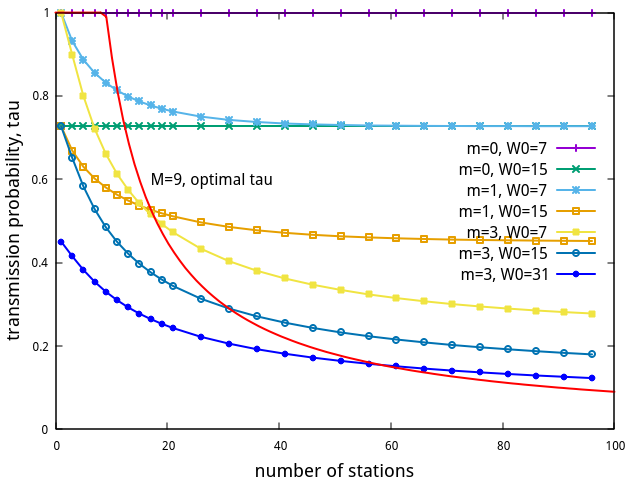
\includegraphics[scale=.54]{./figure/n_tau_perf.png}
\caption{Transmission probability versus number of stations}
\label{fig_n_tau}
\end{figure}

Then, we check the system efficiency and access delay under different parameter sets of $\lbrace m, W_0 \rbrace$. They validate all the rules stated above. 
Firstly, optimal performance is reached under the same system state, i.e. the same $m,W_0$ and the same $n$.
Secondly, smaller $OCW_{min}$ has better performance when $n$ is small.
Thirdly, larger $m$, which means larger $OCW_{max}$, has better performance when $n$ is large. 

Let's take two extreme examples. With smaller $m$ and $OCW_{min}$, performance is pretty well but degrades a lot when $n$ gets larger,
While with larger $m$ and $OCW_{min}$, performance is pretty at large $n$ but much worse for small $n$.
To obtain best performance for $n>M$, we propose to adaptively tune the parameter sets $\lbrace m, OCW_{min}\rbrace$ with large $m$ and small $OCW_{min}$ together with $M$ as large as possible. 

\begin{figure}[!ht]
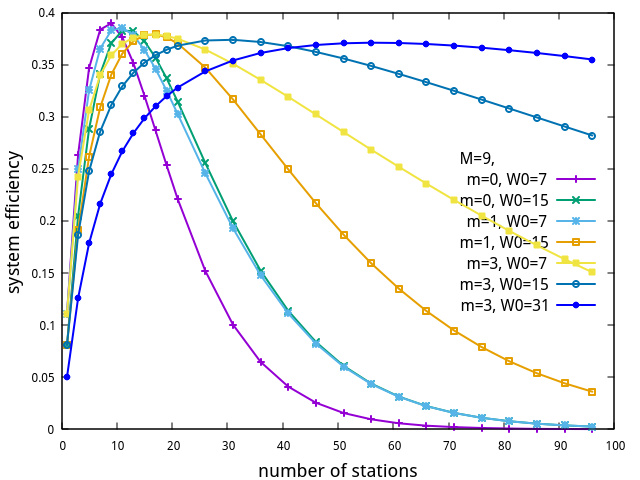
\includegraphics[scale=.54]{./figure/n_eff_perf.png}
\caption{System efficiency versus number of stations}
\label{fig_n_eff}
\end{figure}


\begin{figure}[!ht]
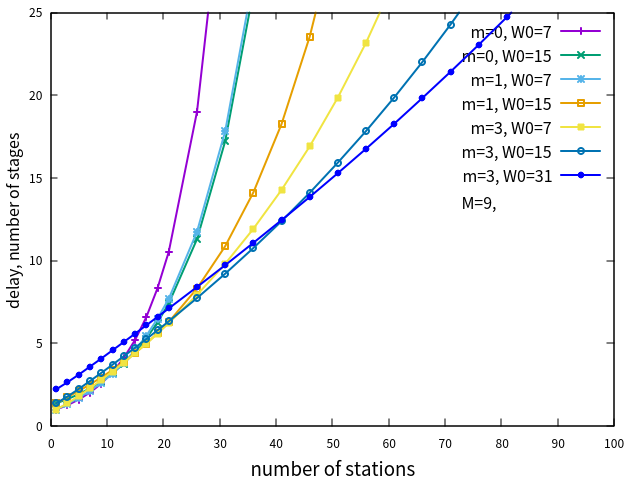
\includegraphics[scale=.54]{./figure/n_delay_perf.png}
\caption{Access delay versus number of stations}
\label{fig_n_delay}
\end{figure}




\subsection{Rules for configuring $\lbrace M,m,OCW_{min} \rbrace$}
Above two previous subsections, we could conclude rules of configuring the parameter set $\lbrace M, m, OCW_{min} \rbrace$ for obtaining best performance for all $n$. 
\begin{itemize}
\item $M$, as large as possible for all $n$.
\item $m, OCW_{min}$
	\begin{itemize}
	\item $n \leq M$, $m = 0$ and small $OCW_{min}$ 
	\item $n > M$, large $m$ and small $OCW_{min}$
	\end{itemize}
\end{itemize}

After we propose the rules of configuring the parameter set $\lbrace M, m, OCW_{min} \rbrace$, we run another analysis with typical group parameter sets which validate our rules.

From figure \ref{fig_n_ns_val}, larger $M = 18$  results in larger $n_s$, number of successful stations in a single stage, than $M=9$. Thus, $M$ is as large as possible.
Then given a $M=18$ as an example, smaller $W_0 = 7$ and larger $m = 7$ have better performance than other parameter sets when $n>M$.

For the system state that $n\leq M$, $n_s$ and access delay of $m=0,W_0 = 7$ is the best case among all the parameter sets. It is because the transmission probability under such condition reaches the optimal value as in figure \ref{fig_n_tau}.  

\begin{figure}[!ht]
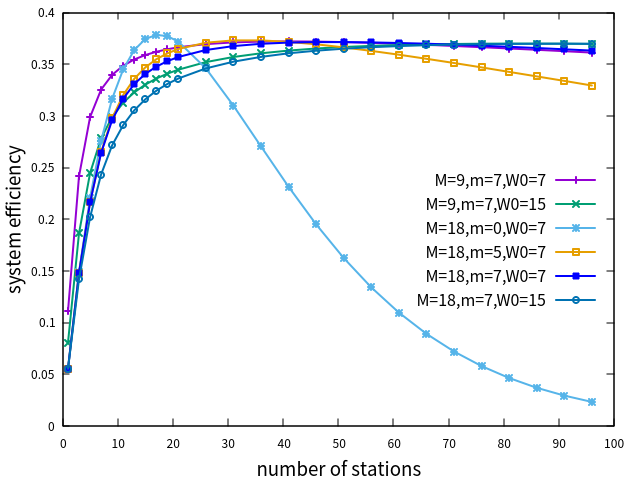
\includegraphics[scale=.54]{./figure/n_rule_eff_perf.png}
\caption{System efficiency versus number of stations}
\label{fig_n_eff_val}
\end{figure}

\begin{figure}[!ht]
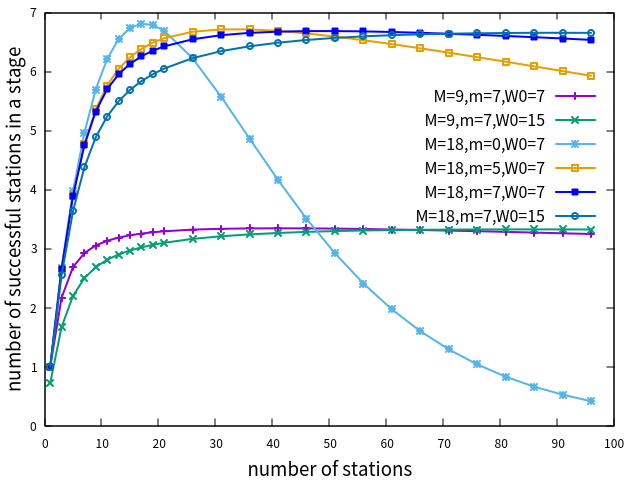
\includegraphics[scale=.54]{./figure/n_rule_ns_perf.png}
\caption{$n_s$ versus number of stations}
\label{fig_n_ns_val}
\end{figure}

\begin{figure}[!ht]
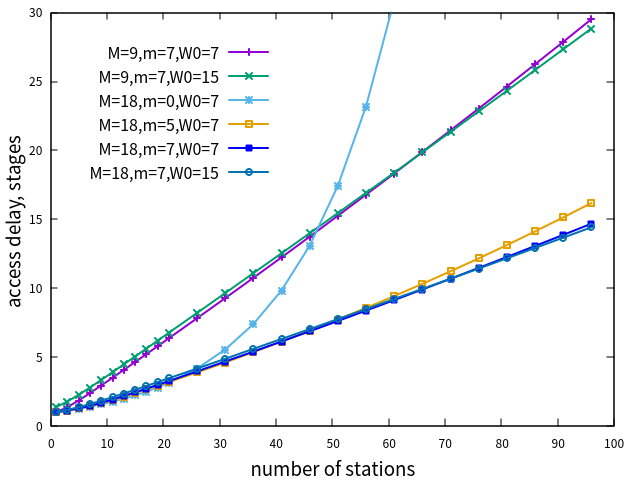
\includegraphics[scale=.54]{./figure/n_rule_delay_perf.png}
\caption{Access Delay versus number of stations}
\label{fig_n_delay_val}
\end{figure}